\documentclass{beamer}
\usepackage{graphics}
\usetheme{Singapore}
\usepackage{graphicx}
\graphicspath{{./figs/}}
\usepackage{amssymb}
\usepackage{amsmath}
\usepackage{amsthm}
\usepackage[dutch]{babel}

\usepackage[absolute,overlay]{textpos} % lelijk

\usepackage{mdframed}

%: Automatische lay-out voor protocollen
\mdfdefinestyle{protocol}{%
    linecolor=gray,
    outerlinewidth=1pt,
    roundcorner=20pt,
    innertopmargin=\baselineskip,
    innerbottommargin=\baselineskip,
    innerrightmargin=20pt,
    innerleftmargin=20pt,
    backgroundcolor=gray!30!white}

\title{Dagelijkse toepassingen van de speltheorie}
\subtitle{Hoe houdt je iedereen tevreden?}
\author{Dani\"el Kuckartz}
\date{\today}

\begin{document}

\newtheorem{step}{Stap}

% Titelpagina
\frame{
    \titlepage
    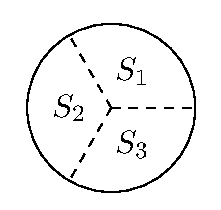
\includegraphics{taart.pdf}
}

% Inhoudsopgave
\frame{
    \frametitle{Inhoudsopgave}
    \tableofcontents
    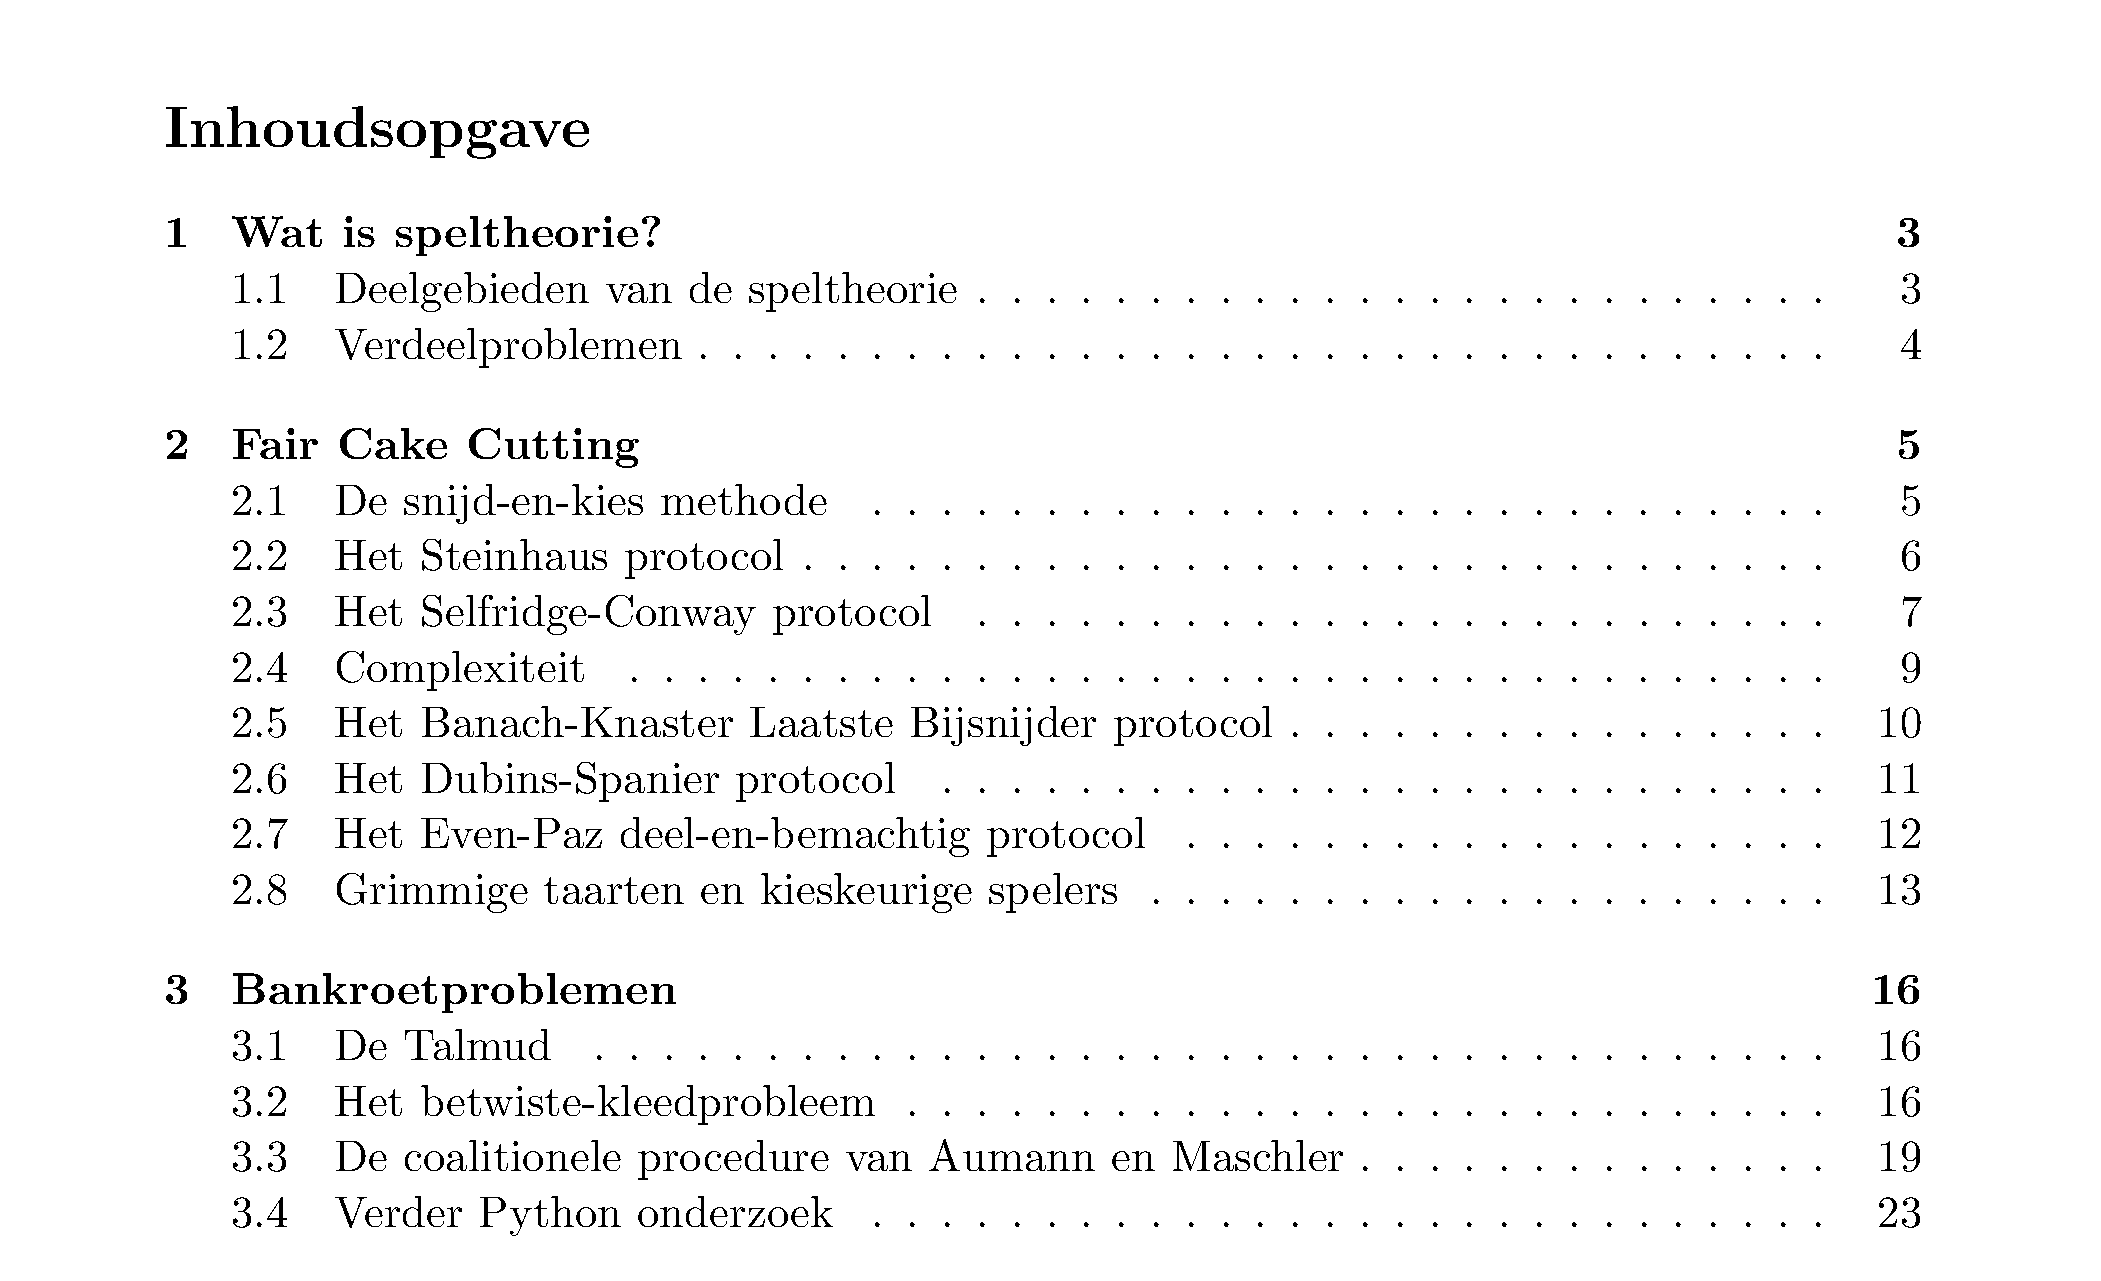
\includegraphics[width=200pt]{inhoudsopgave_pws.pdf}
}

% Introductie
\section{Introductie speltheorie}
\frame{
  \frametitle{Wat is speltheorie?}
      \begin{itemize}%[<+->] 
      \item<1-> Sociaal conflict
      \item<2-> John van Neumann \& Oskar Morgenstein
      \item<3-> Aannames bij de spelers
  \end{itemize}
        %\includegraphics<3->[width=80pt]{cake-cutting-joke}
    \begin{textblock*}{3cm}(6cm,5cm) % {block width} (coords)
    \includegraphics<3->[width=5cm]{cake-cutting-joke.jpg}
    \end{textblock*}
}

% Fair Cake Cutting
\section{Fair Cake Cutting}

\frame{
    \frametitle{Wat is Fair Cake Cutting?}
    
    \begin{itemize}
        \item<1-> Oplossing is een protocol
        \item<2-> Tevreden-zijn
        \begin{itemize}
            \item<2-> $S_1, S_2, \ldots S_n$
            \item<2-> $v_1(X_1)$
        \end{itemize}
     \end{itemize}
     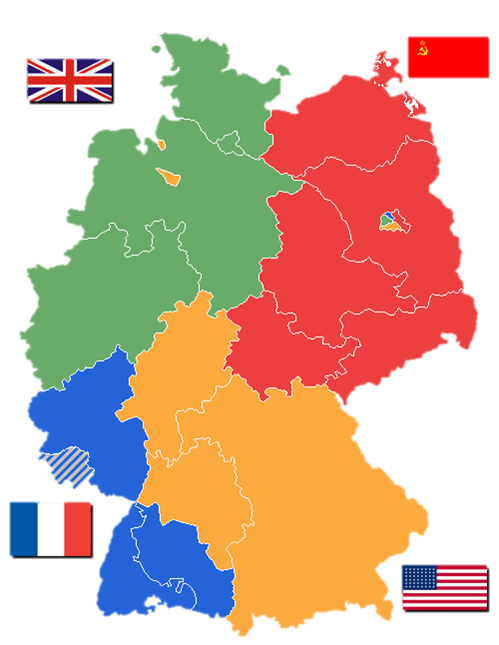
\includegraphics[width=100pt]{berlijn.png}
 }
 
 \frame{
    \frametitle{Klein experiment}
    
        Snijd-en-kies protocol
        \begin{enumerate}[<+->]
            \item $S_1$ maakt een verdeling waarvan hij denkt dat beide delen $\frac{1}{2}$ waard zijn.
            \item$S_2$ kiest een stuk. Als hij denkt dat de stukken ongelijk verdeeld zijn, dan kiest hij het grootste en is tevreden.
            \item$S_1$ neemt het andere stuk. Hij heeft gesneden, dus is tevreden over elk stuk.
        \end{enumerate}
}

\frame{
    \frametitle{Gevonden eisen}

        \begin{description}
            \item[\textbf{jaloezie-vrij}]<1->{Iedereen denkt dat zijn eigen stuk minimaal net zo groot is als de stukken van zijn medespelers \color{red}{$v_i(X_i) \geq v_i(X_j)$ voor $1 \leq i \leq n$ en $1 \leq j \leq n$}}
            \item[\textbf{proportioneel}]<2->{Iedereen denkt het deel te krijgen waar hij recht op heeft  \color{red}{$v_i(X_i) \geq \frac{1}{n}$}}
            \item[\textbf{lage complexiteit}]<3->{Er hoeft zo min mogelijk gesneden te worden. \color{red}{$O(n^2)$}}
        \end{description}
}

\frame{
    \frametitle{Aannames}

        \begin{itemize}[<+->] 
            \item Geen kruimeltjes!
            \item Oneindig deelbaar
        \end{itemize}
}

% Bankroet
\section{Bankroet}

\frame{
    \begin{itemize}
          \item<1-> Tekort
          \item<2-> Betwist kleed
          \item<3> Coalitionele procedure van Aumann \& Maschler
          \begin{itemize}
              \item<3> Maximale uitbetaling
              \item<3> Maximaal verlies
          \end{itemize}
      \end{itemize}
      \includegraphics<2->[width=200pt]{betwist_kleed.pdf}

}

\frame{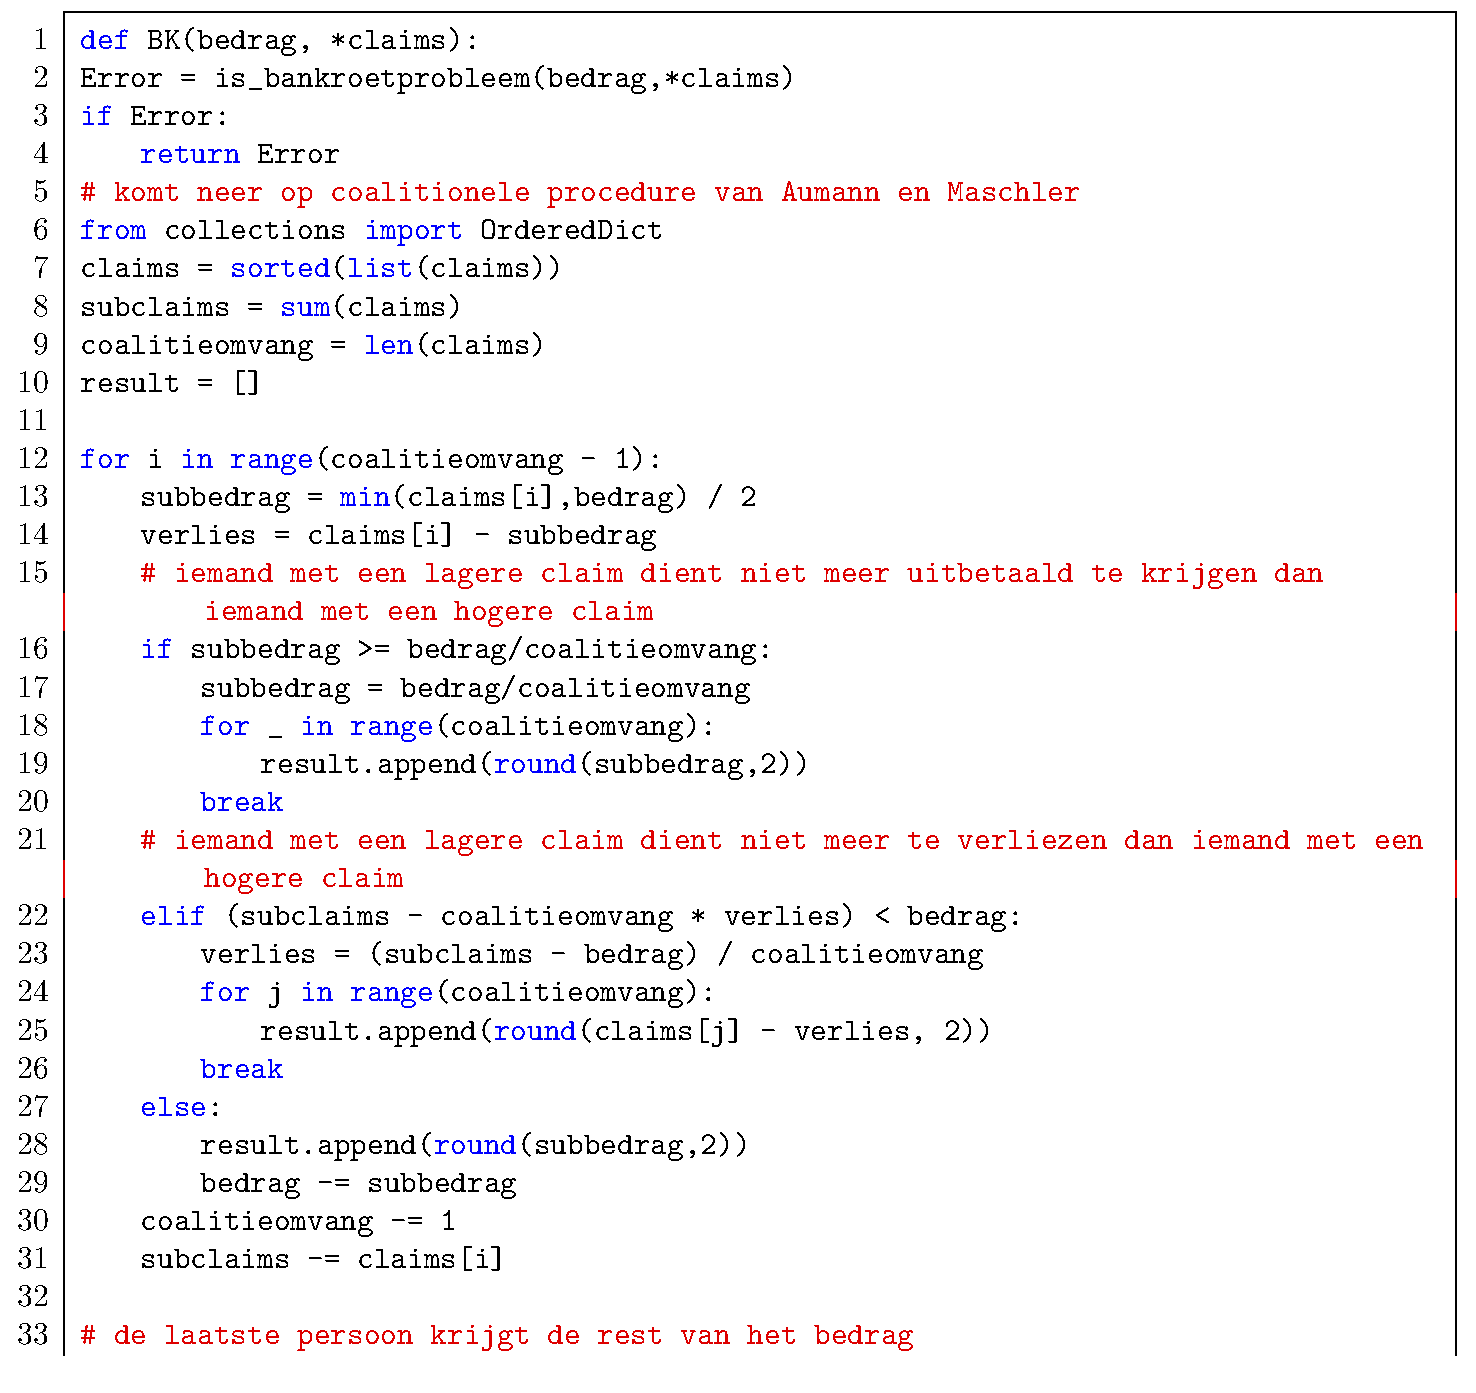
\includegraphics[width=.9\linewidth]{python.pdf}}
\frame{\begin{center}
\includegraphics[width=100pt]{machtig_python.png}\end{center}}

    
\frame{
    \begin{itemize}
          \item Tekort
          \item Betwist kleed
          \item Coalitionele procedure van Aumann \& Maschler
          \begin{itemize}
              \item Maximale uitbetaling
              \item Maximaal verlies
          \end{itemize}
          \item Meerdere goede oplossingen
    \end{itemize}
          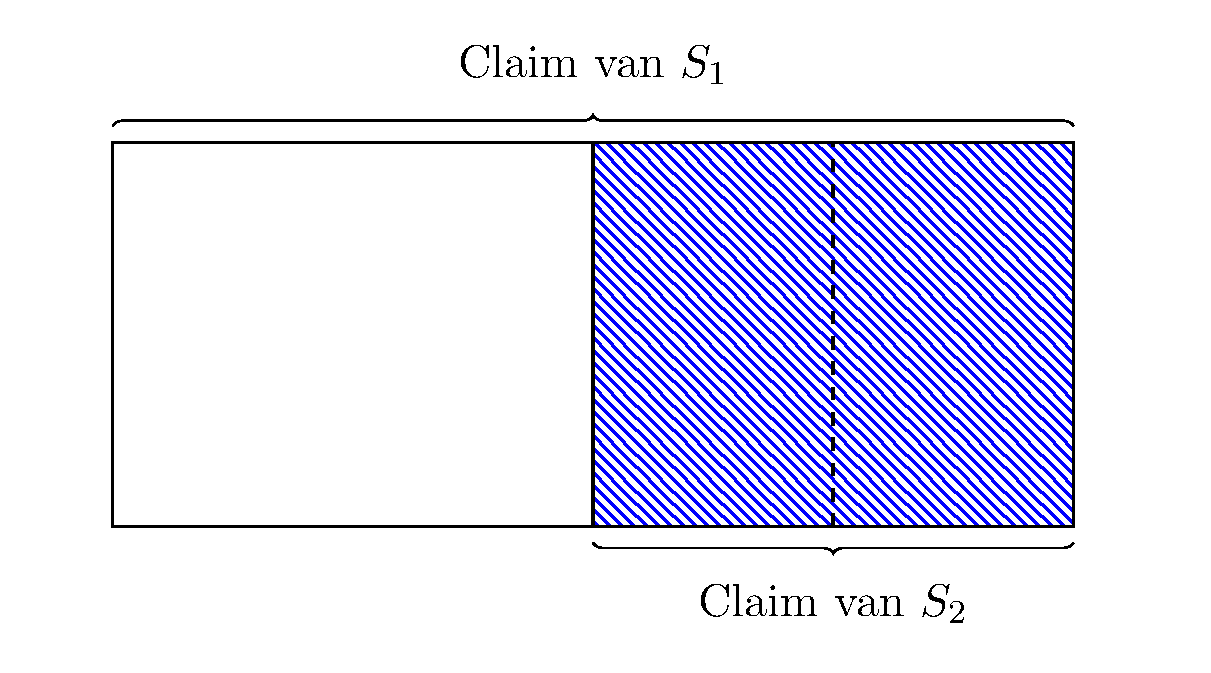
\includegraphics[width=200pt]{betwist_kleed.pdf}
}

\section{Conclusie}

\frame{
    \begin{itemize}[<+->]
          \item<1-> Idealistische aannames
          \begin{itemize}
              \item<1-> Gunfactor
          \end{itemize}          
          \item<2-> Uitdrukken in getallen
          \item<3-> Voorkeur is tijdafhankelijk
          \item<4-> Geen universele beste oplossing
    \end{itemize}
  \includegraphics<1->[width=160pt]{rond_recht.jpg}

}

\frame{
	\centering
          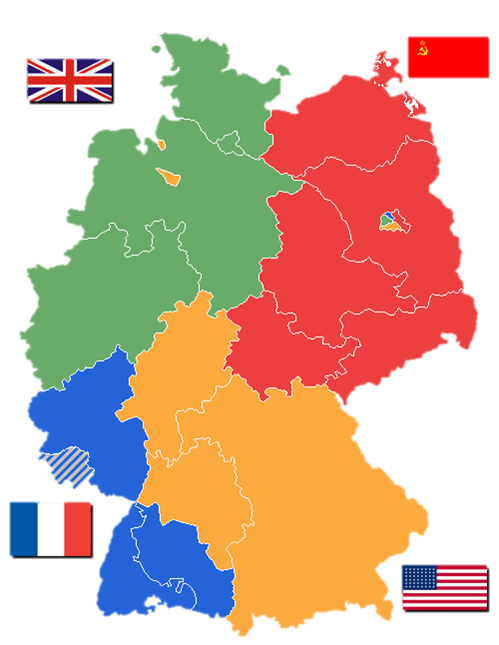
\includegraphics[width=.6\linewidth]{berlijn.png}
}

\frame{
    \begin{itemize}
          \item Idealistische aannames
          \begin{itemize}
              \item Gunfactor
          \end{itemize}          
          \item Uitdrukken in getallen
          \item Voorkeur is tijdafhankelijk
          \item Geen universele beste oplossing
          \item Verder onderzoek nodig
    \end{itemize}
  \includegraphics<1->[width=160pt]{rond_recht.jpg}

}

\end{document}
